% Options for packages loaded elsewhere
\PassOptionsToPackage{unicode}{hyperref}
\PassOptionsToPackage{hyphens}{url}
%
\documentclass[
]{article}
\title{tidytext In\_Class Assignment}
\author{Include Student Name Here}
\date{2023-03-23}

\usepackage{amsmath,amssymb}
\usepackage{lmodern}
\usepackage{iftex}
\ifPDFTeX
  \usepackage[T1]{fontenc}
  \usepackage[utf8]{inputenc}
  \usepackage{textcomp} % provide euro and other symbols
\else % if luatex or xetex
  \usepackage{unicode-math}
  \defaultfontfeatures{Scale=MatchLowercase}
  \defaultfontfeatures[\rmfamily]{Ligatures=TeX,Scale=1}
\fi
% Use upquote if available, for straight quotes in verbatim environments
\IfFileExists{upquote.sty}{\usepackage{upquote}}{}
\IfFileExists{microtype.sty}{% use microtype if available
  \usepackage[]{microtype}
  \UseMicrotypeSet[protrusion]{basicmath} % disable protrusion for tt fonts
}{}
\makeatletter
\@ifundefined{KOMAClassName}{% if non-KOMA class
  \IfFileExists{parskip.sty}{%
    \usepackage{parskip}
  }{% else
    \setlength{\parindent}{0pt}
    \setlength{\parskip}{6pt plus 2pt minus 1pt}}
}{% if KOMA class
  \KOMAoptions{parskip=half}}
\makeatother
\usepackage{xcolor}
\IfFileExists{xurl.sty}{\usepackage{xurl}}{} % add URL line breaks if available
\IfFileExists{bookmark.sty}{\usepackage{bookmark}}{\usepackage{hyperref}}
\hypersetup{
  pdftitle={tidytext In\_Class Assignment},
  pdfauthor={Include Student Name Here},
  hidelinks,
  pdfcreator={LaTeX via pandoc}}
\urlstyle{same} % disable monospaced font for URLs
\usepackage[margin=1in]{geometry}
\usepackage{color}
\usepackage{fancyvrb}
\newcommand{\VerbBar}{|}
\newcommand{\VERB}{\Verb[commandchars=\\\{\}]}
\DefineVerbatimEnvironment{Highlighting}{Verbatim}{commandchars=\\\{\}}
% Add ',fontsize=\small' for more characters per line
\usepackage{framed}
\definecolor{shadecolor}{RGB}{248,248,248}
\newenvironment{Shaded}{\begin{snugshade}}{\end{snugshade}}
\newcommand{\AlertTok}[1]{\textcolor[rgb]{0.94,0.16,0.16}{#1}}
\newcommand{\AnnotationTok}[1]{\textcolor[rgb]{0.56,0.35,0.01}{\textbf{\textit{#1}}}}
\newcommand{\AttributeTok}[1]{\textcolor[rgb]{0.77,0.63,0.00}{#1}}
\newcommand{\BaseNTok}[1]{\textcolor[rgb]{0.00,0.00,0.81}{#1}}
\newcommand{\BuiltInTok}[1]{#1}
\newcommand{\CharTok}[1]{\textcolor[rgb]{0.31,0.60,0.02}{#1}}
\newcommand{\CommentTok}[1]{\textcolor[rgb]{0.56,0.35,0.01}{\textit{#1}}}
\newcommand{\CommentVarTok}[1]{\textcolor[rgb]{0.56,0.35,0.01}{\textbf{\textit{#1}}}}
\newcommand{\ConstantTok}[1]{\textcolor[rgb]{0.00,0.00,0.00}{#1}}
\newcommand{\ControlFlowTok}[1]{\textcolor[rgb]{0.13,0.29,0.53}{\textbf{#1}}}
\newcommand{\DataTypeTok}[1]{\textcolor[rgb]{0.13,0.29,0.53}{#1}}
\newcommand{\DecValTok}[1]{\textcolor[rgb]{0.00,0.00,0.81}{#1}}
\newcommand{\DocumentationTok}[1]{\textcolor[rgb]{0.56,0.35,0.01}{\textbf{\textit{#1}}}}
\newcommand{\ErrorTok}[1]{\textcolor[rgb]{0.64,0.00,0.00}{\textbf{#1}}}
\newcommand{\ExtensionTok}[1]{#1}
\newcommand{\FloatTok}[1]{\textcolor[rgb]{0.00,0.00,0.81}{#1}}
\newcommand{\FunctionTok}[1]{\textcolor[rgb]{0.00,0.00,0.00}{#1}}
\newcommand{\ImportTok}[1]{#1}
\newcommand{\InformationTok}[1]{\textcolor[rgb]{0.56,0.35,0.01}{\textbf{\textit{#1}}}}
\newcommand{\KeywordTok}[1]{\textcolor[rgb]{0.13,0.29,0.53}{\textbf{#1}}}
\newcommand{\NormalTok}[1]{#1}
\newcommand{\OperatorTok}[1]{\textcolor[rgb]{0.81,0.36,0.00}{\textbf{#1}}}
\newcommand{\OtherTok}[1]{\textcolor[rgb]{0.56,0.35,0.01}{#1}}
\newcommand{\PreprocessorTok}[1]{\textcolor[rgb]{0.56,0.35,0.01}{\textit{#1}}}
\newcommand{\RegionMarkerTok}[1]{#1}
\newcommand{\SpecialCharTok}[1]{\textcolor[rgb]{0.00,0.00,0.00}{#1}}
\newcommand{\SpecialStringTok}[1]{\textcolor[rgb]{0.31,0.60,0.02}{#1}}
\newcommand{\StringTok}[1]{\textcolor[rgb]{0.31,0.60,0.02}{#1}}
\newcommand{\VariableTok}[1]{\textcolor[rgb]{0.00,0.00,0.00}{#1}}
\newcommand{\VerbatimStringTok}[1]{\textcolor[rgb]{0.31,0.60,0.02}{#1}}
\newcommand{\WarningTok}[1]{\textcolor[rgb]{0.56,0.35,0.01}{\textbf{\textit{#1}}}}
\usepackage{graphicx}
\makeatletter
\def\maxwidth{\ifdim\Gin@nat@width>\linewidth\linewidth\else\Gin@nat@width\fi}
\def\maxheight{\ifdim\Gin@nat@height>\textheight\textheight\else\Gin@nat@height\fi}
\makeatother
% Scale images if necessary, so that they will not overflow the page
% margins by default, and it is still possible to overwrite the defaults
% using explicit options in \includegraphics[width, height, ...]{}
\setkeys{Gin}{width=\maxwidth,height=\maxheight,keepaspectratio}
% Set default figure placement to htbp
\makeatletter
\def\fps@figure{htbp}
\makeatother
\setlength{\emergencystretch}{3em} % prevent overfull lines
\providecommand{\tightlist}{%
  \setlength{\itemsep}{0pt}\setlength{\parskip}{0pt}}
\setcounter{secnumdepth}{-\maxdimen} % remove section numbering
\ifLuaTeX
  \usepackage{selnolig}  % disable illegal ligatures
\fi

\begin{document}
\maketitle

\hypertarget{the-questions-in-this-markdown-must-be-answered-using-the-tidyr-and-dplyr-packages-functions.}{%
\subsection{The questions in this markdown must be answered using the
tidyr and dplyr packages'
functions.}\label{the-questions-in-this-markdown-must-be-answered-using-the-tidyr-and-dplyr-packages-functions.}}

\hypertarget{the-tidyverse-functionality-is-greatly-enhanced-using-the-pipes-from-magrittr}{%
\paragraph{The tidyverse functionality is greatly enhanced using the
pipes (\%\textgreater\% from
magrittr)}\label{the-tidyverse-functionality-is-greatly-enhanced-using-the-pipes-from-magrittr}}

\hypertarget{load-the-required-packages-before-starting-the-assignment.}{%
\paragraph{Load the required packages before starting the
assignment.}\label{load-the-required-packages-before-starting-the-assignment.}}

\hypertarget{questions-1-through-11-are-related-to-tidyr-with-one-exception-of-using-a-base-function---replace}{%
\paragraph{Questions 1 through 11 are related to tidyr (with one
exception of using a base function -
``replace'')}\label{questions-1-through-11-are-related-to-tidyr-with-one-exception-of-using-a-base-function---replace}}

\hypertarget{questions-12-through-11-are-related-to-tidyr-with-one-exception-of-using-a-base-function---replace}{%
\paragraph{Questions 12 through 11 are related to tidyr (with one
exception of using a base function -
``replace'')}\label{questions-12-through-11-are-related-to-tidyr-with-one-exception-of-using-a-base-function---replace}}

\begin{Shaded}
\begin{Highlighting}[]
\CommentTok{\# Take a look at the religious income dataset, relig\_income and answer if the dataset is a tidy dataset.}
\FunctionTok{library}\NormalTok{(tidyverse)}
\end{Highlighting}
\end{Shaded}

\begin{verbatim}
## Warning: package 'tidyverse' was built under R version 4.1.3
\end{verbatim}

\begin{verbatim}
## -- Attaching packages --------------------------------------- tidyverse 1.3.2 --
## v ggplot2 3.4.0     v purrr   1.0.1
## v tibble  3.1.8     v dplyr   1.1.0
## v tidyr   1.3.0     v stringr 1.5.0
## v readr   2.1.4     v forcats 1.0.0
\end{verbatim}

\begin{verbatim}
## Warning: package 'ggplot2' was built under R version 4.1.3
\end{verbatim}

\begin{verbatim}
## Warning: package 'tibble' was built under R version 4.1.3
\end{verbatim}

\begin{verbatim}
## Warning: package 'tidyr' was built under R version 4.1.3
\end{verbatim}

\begin{verbatim}
## Warning: package 'readr' was built under R version 4.1.3
\end{verbatim}

\begin{verbatim}
## Warning: package 'purrr' was built under R version 4.1.3
\end{verbatim}

\begin{verbatim}
## Warning: package 'dplyr' was built under R version 4.1.3
\end{verbatim}

\begin{verbatim}
## Warning: package 'stringr' was built under R version 4.1.3
\end{verbatim}

\begin{verbatim}
## Warning: package 'forcats' was built under R version 4.1.3
\end{verbatim}

\begin{verbatim}
## -- Conflicts ------------------------------------------ tidyverse_conflicts() --
## x dplyr::filter() masks stats::filter()
## x dplyr::lag()    masks stats::lag()
\end{verbatim}

\begin{Shaded}
\begin{Highlighting}[]
\FunctionTok{View}\NormalTok{(relig\_income)}

\CommentTok{\# If not, why is it not a tidy dataset?}
\CommentTok{\#\textquotesingle{} it\textquotesingle{}s not a tidy dataset, because income should be under 1 column only for the data set to be a tidy dataset}

\CommentTok{\# Tidy the dataset using pivot\_longer transformation.}
\NormalTok{relig\_income }\SpecialCharTok{\%\textgreater{}\%}
\FunctionTok{pivot\_longer}\NormalTok{(}\AttributeTok{cols =} \SpecialCharTok{{-}}\NormalTok{religion,}
             \AttributeTok{names\_to =} \StringTok{"income\_range"}\NormalTok{,}
             \AttributeTok{values\_to =} \StringTok{"income"}\NormalTok{)}
\end{Highlighting}
\end{Shaded}

\begin{verbatim}
## # A tibble: 180 x 3
##    religion income_range       income
##    <chr>    <chr>               <dbl>
##  1 Agnostic <$10k                  27
##  2 Agnostic $10-20k                34
##  3 Agnostic $20-30k                60
##  4 Agnostic $30-40k                81
##  5 Agnostic $40-50k                76
##  6 Agnostic $50-75k               137
##  7 Agnostic $75-100k              122
##  8 Agnostic $100-150k             109
##  9 Agnostic >150k                  84
## 10 Agnostic Don't know/refused     96
## # ... with 170 more rows
\end{verbatim}

\begin{Shaded}
\begin{Highlighting}[]
\FunctionTok{library}\NormalTok{(tidyverse)}
\NormalTok{student\_scores }\OtherTok{\textless{}{-}} \FunctionTok{tribble}\NormalTok{(}
  \SpecialCharTok{\textasciitilde{}}\NormalTok{name, }\SpecialCharTok{\textasciitilde{}}\NormalTok{bus101, }\SpecialCharTok{\textasciitilde{}}\NormalTok{bus201, }\SpecialCharTok{\textasciitilde{}}\NormalTok{eco101, }\SpecialCharTok{\textasciitilde{}}\NormalTok{fin101, }
  \StringTok{"Billy"}\NormalTok{, }\DecValTok{90}\NormalTok{, }\DecValTok{96}\NormalTok{, }\DecValTok{70}\NormalTok{, }\DecValTok{76}\NormalTok{, }
  \StringTok{"Suzy"}\NormalTok{, }\DecValTok{82}\NormalTok{, }\DecValTok{76}\NormalTok{, }\DecValTok{78}\NormalTok{, }\DecValTok{86}\NormalTok{,}
  \StringTok{"Lionel"}\NormalTok{, }\DecValTok{68}\NormalTok{, }\DecValTok{56}\NormalTok{, }\DecValTok{79}\NormalTok{, }\DecValTok{82}\NormalTok{, }
  \StringTok{"Jenny"}\NormalTok{, }\DecValTok{72}\NormalTok{, }\DecValTok{96}\NormalTok{, }\DecValTok{71}\NormalTok{, }\DecValTok{90}\NormalTok{,}
\NormalTok{)}

\CommentTok{\# Merge the Business courses into a single column with the name "Business Courses" and the corresponding values from their respective column names. While saving the values, only use numeric course numbers 101 and 201. }
\CommentTok{\# Use names\_prefix to suppress character values from the column names }
\NormalTok{student\_scores }\SpecialCharTok{\%\textgreater{}\%}
\FunctionTok{pivot\_longer}\NormalTok{(}\AttributeTok{cols =} \FunctionTok{c}\NormalTok{(}\StringTok{"bus101"}\NormalTok{, }\StringTok{"bus201"}\NormalTok{),}
             \AttributeTok{names\_to =} \StringTok{"Business Courses"}\NormalTok{,}
             \AttributeTok{values\_to =} \StringTok{"Score"}\NormalTok{,}
             \AttributeTok{names\_prefix =} \StringTok{"bus"}\NormalTok{)}
\end{Highlighting}
\end{Shaded}

\begin{verbatim}
## # A tibble: 8 x 5
##   name   eco101 fin101 `Business Courses` Score
##   <chr>   <dbl>  <dbl> <chr>              <dbl>
## 1 Billy      70     76 101                   90
## 2 Billy      70     76 201                   96
## 3 Suzy       78     86 101                   82
## 4 Suzy       78     86 201                   76
## 5 Lionel     79     82 101                   68
## 6 Lionel     79     82 201                   56
## 7 Jenny      71     90 101                   72
## 8 Jenny      71     90 201                   96
\end{verbatim}

\begin{Shaded}
\begin{Highlighting}[]
\CommentTok{\# Use the names pattern function to split required values. The value "bus101" should be split such that "bus" appears in the "major" column and "101" appears in the "course id" column.}
\CommentTok{\# Use names\_pattern to specify how each column should be split into the specified number of columns.}
\CommentTok{\# Use names\_to to provide the names of the new columns. }
\NormalTok{student\_scores }\SpecialCharTok{\%\textgreater{}\%}
\FunctionTok{pivot\_longer}\NormalTok{(}\AttributeTok{cols =} \SpecialCharTok{{-}}\NormalTok{name,}
             \AttributeTok{names\_to =} \FunctionTok{c}\NormalTok{(}\StringTok{"Major"}\NormalTok{,}\StringTok{"Courses"}\NormalTok{),}
             \AttributeTok{values\_to =} \StringTok{"Score"}\NormalTok{,}
             \AttributeTok{names\_pattern =} \StringTok{"([a{-}z]\{3\})([0{-}9]\{3\})"}\NormalTok{)}
\end{Highlighting}
\end{Shaded}

\begin{verbatim}
## # A tibble: 16 x 4
##    name   Major Courses Score
##    <chr>  <chr> <chr>   <dbl>
##  1 Billy  bus   101        90
##  2 Billy  bus   201        96
##  3 Billy  eco   101        70
##  4 Billy  fin   101        76
##  5 Suzy   bus   101        82
##  6 Suzy   bus   201        76
##  7 Suzy   eco   101        78
##  8 Suzy   fin   101        86
##  9 Lionel bus   101        68
## 10 Lionel bus   201        56
## 11 Lionel eco   101        79
## 12 Lionel fin   101        82
## 13 Jenny  bus   101        72
## 14 Jenny  bus   201        96
## 15 Jenny  eco   101        71
## 16 Jenny  fin   101        90
\end{verbatim}

\begin{Shaded}
\begin{Highlighting}[]
\CommentTok{\#[aeiou896] \textless{}{-} whatever matches what\textquotesingle{}s in between the brakets}
\CommentTok{\# \{3,4\} \textless{}{-} user for cases like bus101, buss101. min is 3 and max is 4}
\end{Highlighting}
\end{Shaded}

\begin{Shaded}
\begin{Highlighting}[]
\CommentTok{\# Take a look at each of these tables and answer which table is tidy and which tables are not tidy. (Check!!!)}
\CommentTok{\# table1: tidy }
\CommentTok{\# table2: not tidy (has cases and population under 1 column. They should be seperate)}
\CommentTok{\# table3: not tidy (has compound values)}
\CommentTok{\# table4a: not tidy (has year in separate columns)}
\CommentTok{\# table4b: not tidy (has year in separate columns)}

\CommentTok{\#\textquotesingle{}table1, table2, table3, table4a, table4b, and table5 all display the number of  TB cases documented by the World Health Organization in Afghanistan, Brazil, and China between 1999 and 2000. The data contains values associated with four variables (country, year, cases, and population), but each table organizes the values in a different layout. }
\CommentTok{\#\textquotesingle{}The data is a subset of the data contained in the World Health Organization Global Tuberculosis Report}
\end{Highlighting}
\end{Shaded}

\begin{Shaded}
\begin{Highlighting}[]
\CommentTok{\# Using table2, split the "type" column into two columns, with cases and population as column names. User pivot\_wider() function  }
\NormalTok{table2 }\SpecialCharTok{\%\textgreater{}\%}
\FunctionTok{pivot\_wider}\NormalTok{(}\AttributeTok{names\_from =} \StringTok{"type"}\NormalTok{,}
             \AttributeTok{values\_from =} \StringTok{"count"}\NormalTok{)}
\end{Highlighting}
\end{Shaded}

\begin{verbatim}
## # A tibble: 6 x 4
##   country      year  cases population
##   <chr>       <dbl>  <dbl>      <dbl>
## 1 Afghanistan  1999    745   19987071
## 2 Afghanistan  2000   2666   20595360
## 3 Brazil       1999  37737  172006362
## 4 Brazil       2000  80488  174504898
## 5 China        1999 212258 1272915272
## 6 China        2000 213766 1280428583
\end{verbatim}

\begin{Shaded}
\begin{Highlighting}[]
\CommentTok{\# Using table3, separate the rate column into two columns, cases and population. Use separate() function }
\NormalTok{table3 }\SpecialCharTok{\%\textgreater{}\%}
  \FunctionTok{separate}\NormalTok{(}\AttributeTok{col =} \StringTok{"rate"}\NormalTok{,}
           \AttributeTok{into =} \FunctionTok{c}\NormalTok{(}\StringTok{"Cases"}\NormalTok{, }\StringTok{"Population"}\NormalTok{),}
           \AttributeTok{sep =} \StringTok{"/"}\NormalTok{)}
\end{Highlighting}
\end{Shaded}

\begin{verbatim}
## # A tibble: 6 x 4
##   country      year Cases  Population
##   <chr>       <dbl> <chr>  <chr>     
## 1 Afghanistan  1999 745    19987071  
## 2 Afghanistan  2000 2666   20595360  
## 3 Brazil       1999 37737  172006362 
## 4 Brazil       2000 80488  174504898 
## 5 China        1999 212258 1272915272
## 6 China        2000 213766 1280428583
\end{verbatim}

\begin{Shaded}
\begin{Highlighting}[]
\NormalTok{student\_details }\OtherTok{\textless{}{-}} \FunctionTok{tribble}\NormalTok{(}
  \SpecialCharTok{\textasciitilde{}}\NormalTok{name, }\SpecialCharTok{\textasciitilde{}}\NormalTok{day, }\SpecialCharTok{\textasciitilde{}}\NormalTok{month, }\SpecialCharTok{\textasciitilde{}}\NormalTok{year, }\SpecialCharTok{\textasciitilde{}}\StringTok{"pass/fail"}\NormalTok{, }
  \StringTok{"Billy"}\NormalTok{, }\DecValTok{15}\NormalTok{, }\DecValTok{04}\NormalTok{, }\DecValTok{96}\NormalTok{, }\StringTok{"Pass"}\NormalTok{, }
  \StringTok{"Suzy"}\NormalTok{, }\DecValTok{21}\NormalTok{, }\DecValTok{10}\NormalTok{, }\DecValTok{98}\NormalTok{, }\StringTok{"Fail"}\NormalTok{,}
  \StringTok{"Lionel"}\NormalTok{, }\DecValTok{27}\NormalTok{, }\DecValTok{09}\NormalTok{, }\DecValTok{97}\NormalTok{, }\StringTok{"Pass"}\NormalTok{, }
  \StringTok{"Jenny"}\NormalTok{, }\DecValTok{01}\NormalTok{, }\DecValTok{04}\NormalTok{, }\DecValTok{99}\NormalTok{, }\StringTok{"Pass"}
\NormalTok{)}

\NormalTok{student\_details }\SpecialCharTok{\%\textgreater{}\%}
\FunctionTok{unite}\NormalTok{(}\AttributeTok{col =} \StringTok{"DOB"}\NormalTok{,}
      \FunctionTok{c}\NormalTok{(day, month, year),}
      \AttributeTok{sep =} \StringTok{"/"}\NormalTok{)}
\end{Highlighting}
\end{Shaded}

\begin{verbatim}
## # A tibble: 4 x 3
##   name   DOB      `pass/fail`
##   <chr>  <chr>    <chr>      
## 1 Billy  15/4/96  Pass       
## 2 Suzy   21/10/98 Fail       
## 3 Lionel 27/9/97  Pass       
## 4 Jenny  1/4/99   Pass
\end{verbatim}

\begin{Shaded}
\begin{Highlighting}[]
\CommentTok{\# ... \textless{}{-} positional parameter}
\end{Highlighting}
\end{Shaded}

\begin{Shaded}
\begin{Highlighting}[]
\CommentTok{\# Use the complete() function of tidyr to insert rows with all possible combinations of name and course columns. }
\NormalTok{student\_scores }\OtherTok{\textless{}{-}} \FunctionTok{tribble}\NormalTok{( }
  \SpecialCharTok{\textasciitilde{}}\NormalTok{name, }\SpecialCharTok{\textasciitilde{}}\NormalTok{course, }\SpecialCharTok{\textasciitilde{}}\NormalTok{score, }
  \StringTok{"Billy"}\NormalTok{, }\StringTok{"bus101"}\NormalTok{, }\DecValTok{90}\NormalTok{,}
  \StringTok{"Billy"}\NormalTok{, }\StringTok{"fin101"}\NormalTok{, }\DecValTok{76}\NormalTok{,}
  \StringTok{"Suzy"}\NormalTok{, }\StringTok{"bus101"}\NormalTok{, }\DecValTok{82}\NormalTok{,}
  \StringTok{"Suzy"}\NormalTok{, }\StringTok{"bus201"}\NormalTok{, }\DecValTok{76}\NormalTok{,}
  \StringTok{"Suzy"}\NormalTok{, }\StringTok{"eco101"}\NormalTok{, }\DecValTok{78}\NormalTok{,}
  \StringTok{"Suzy"}\NormalTok{, }\StringTok{"fin101"}\NormalTok{, }\DecValTok{86}\NormalTok{,}
  \StringTok{"Lionel"}\NormalTok{, }\StringTok{"bus101"}\NormalTok{, }\DecValTok{68}\NormalTok{,}
  \StringTok{"Lionel"}\NormalTok{, }\StringTok{"bus201"}\NormalTok{, }\DecValTok{56}\NormalTok{,}
  \StringTok{"Lionel"}\NormalTok{, }\StringTok{"eco101"}\NormalTok{, }\DecValTok{79}\NormalTok{,}
  \StringTok{"Lionel"}\NormalTok{, }\StringTok{"fin101"}\NormalTok{, }\ConstantTok{NA}\NormalTok{ )}

\CommentTok{\# make the number of entries consistent by name and course}
\NormalTok{student\_scores }\SpecialCharTok{\%\textgreater{}\%}
\FunctionTok{complete}\NormalTok{(name, course)}
\end{Highlighting}
\end{Shaded}

\begin{verbatim}
## # A tibble: 12 x 3
##    name   course score
##    <chr>  <chr>  <dbl>
##  1 Billy  bus101    90
##  2 Billy  bus201    NA
##  3 Billy  eco101    NA
##  4 Billy  fin101    76
##  5 Lionel bus101    68
##  6 Lionel bus201    56
##  7 Lionel eco101    79
##  8 Lionel fin101    NA
##  9 Suzy   bus101    82
## 10 Suzy   bus201    76
## 11 Suzy   eco101    78
## 12 Suzy   fin101    86
\end{verbatim}

\begin{Shaded}
\begin{Highlighting}[]
\CommentTok{\# Find the indexes or row numbers of sleep dataset that has negative numbers in extra column }
\CommentTok{\# Make sure that the indexes are of integer type (Numeric)}
\CommentTok{\# Use replace function to replace the negative numbers with 0}

\CommentTok{\#replace example}
\NormalTok{vec1 }\OtherTok{\textless{}{-}} \DecValTok{1}\SpecialCharTok{:}\DecValTok{10}
\FunctionTok{replace}\NormalTok{(vec1, }\FunctionTok{c}\NormalTok{(}\DecValTok{3}\NormalTok{,}\DecValTok{4}\NormalTok{), }\DecValTok{99}\NormalTok{)}
\end{Highlighting}
\end{Shaded}

\begin{verbatim}
##  [1]  1  2 99 99  5  6  7  8  9 10
\end{verbatim}

\begin{Shaded}
\begin{Highlighting}[]
\FunctionTok{replace}\NormalTok{(}
\NormalTok{  sleep}\SpecialCharTok{$}\NormalTok{extra,}
  \FunctionTok{as.integer}\NormalTok{(}\FunctionTok{row.names}\NormalTok{(sleep[sleep}\SpecialCharTok{$}\NormalTok{extra }\SpecialCharTok{\textless{}} \DecValTok{0}\NormalTok{,])),}
  \DecValTok{0}\NormalTok{)}
\end{Highlighting}
\end{Shaded}

\begin{verbatim}
##  [1] 0.7 0.0 0.0 0.0 0.0 3.4 3.7 0.8 0.0 2.0 1.9 0.8 1.1 0.1 0.0 4.4 5.5 1.6 4.6
## [20] 3.4
\end{verbatim}

\begin{Shaded}
\begin{Highlighting}[]
\CommentTok{\#another way}
\CommentTok{\#sleep \%\textgreater{}\%}
 \CommentTok{\# mutate(extra = ifelse(extra \textless{} 0,], 0, extra))}
\end{Highlighting}
\end{Shaded}

\begin{Shaded}
\begin{Highlighting}[]
\NormalTok{student\_scores }\OtherTok{\textless{}{-}} \FunctionTok{tribble}\NormalTok{(}
  \SpecialCharTok{\textasciitilde{}}\NormalTok{name, }\SpecialCharTok{\textasciitilde{}}\NormalTok{course, }\SpecialCharTok{\textasciitilde{}}\NormalTok{score,}

  \StringTok{"Billy"}\NormalTok{,  }\StringTok{"bus101"}\NormalTok{, }\DecValTok{90}\NormalTok{,}
  \StringTok{"Billy"}\NormalTok{,  }\StringTok{"bus201"}\NormalTok{, }\ConstantTok{NA}\NormalTok{,}
  \StringTok{"Billy"}\NormalTok{, }\StringTok{"eco101"}\NormalTok{, }\ConstantTok{NA}\NormalTok{,}
  \StringTok{"Billy"}\NormalTok{, }\StringTok{"fin101"}\NormalTok{, }\DecValTok{76}\NormalTok{,}
  \StringTok{"Lionel"}\NormalTok{, }\StringTok{"bus101"}\NormalTok{, }\DecValTok{68}\NormalTok{,}
  \StringTok{"Lionel"}\NormalTok{, }\StringTok{"bus201"}\NormalTok{, }\DecValTok{56}\NormalTok{,}
  \StringTok{"Lionel"}\NormalTok{, }\StringTok{"eco101"}\NormalTok{, }\DecValTok{79}\NormalTok{,}
  \StringTok{"Lionel"}\NormalTok{, }\StringTok{"fin101"}\NormalTok{, }\ConstantTok{NA}\NormalTok{,}
  \StringTok{"Suzy"}\NormalTok{, }\StringTok{"bus101"}\NormalTok{, }\DecValTok{82}\NormalTok{,}
  \StringTok{"Suzy"}\NormalTok{, }\StringTok{"bus201"}\NormalTok{, }\DecValTok{76}\NormalTok{,}
  \StringTok{"Suzy"}\NormalTok{, }\StringTok{"eco101"}\NormalTok{, }\DecValTok{78}\NormalTok{,}
  \StringTok{"Suzy"}\NormalTok{, }\StringTok{"fin101"}\NormalTok{, }\DecValTok{86}
\NormalTok{)}

\NormalTok{student\_scores }\SpecialCharTok{\%\textgreater{}\%}
  \FunctionTok{replace\_na}\NormalTok{(}\FunctionTok{list}\NormalTok{(}\AttributeTok{score =} \FloatTok{0.0}\NormalTok{))}
\end{Highlighting}
\end{Shaded}

\begin{verbatim}
## # A tibble: 12 x 3
##    name   course score
##    <chr>  <chr>  <dbl>
##  1 Billy  bus101    90
##  2 Billy  bus201     0
##  3 Billy  eco101     0
##  4 Billy  fin101    76
##  5 Lionel bus101    68
##  6 Lionel bus201    56
##  7 Lionel eco101    79
##  8 Lionel fin101     0
##  9 Suzy   bus101    82
## 10 Suzy   bus201    76
## 11 Suzy   eco101    78
## 12 Suzy   fin101    86
\end{verbatim}

\begin{Shaded}
\begin{Highlighting}[]
\CommentTok{\# we can impute missing values with mean values mean(x)}
\end{Highlighting}
\end{Shaded}

\hypertarget{dplyr-functions}{%
\paragraph{dplyr functions}\label{dplyr-functions}}

\begin{Shaded}
\begin{Highlighting}[]
\NormalTok{superheroes }\OtherTok{\textless{}{-}}\NormalTok{ tibble}\SpecialCharTok{::}\FunctionTok{tribble}\NormalTok{(}
       \SpecialCharTok{\textasciitilde{}}\NormalTok{name, }\SpecialCharTok{\textasciitilde{}}\NormalTok{alignment,  }\SpecialCharTok{\textasciitilde{}}\NormalTok{gender,          }\SpecialCharTok{\textasciitilde{}}\NormalTok{publisher,}
   \StringTok{"Magneto"}\NormalTok{,      }\StringTok{"bad"}\NormalTok{,   }\StringTok{"male"}\NormalTok{,            }\StringTok{"Marvel"}\NormalTok{,}
     \StringTok{"Storm"}\NormalTok{,     }\StringTok{"good"}\NormalTok{, }\StringTok{"female"}\NormalTok{,            }\StringTok{"Marvel"}\NormalTok{,}
  \StringTok{"Mystique"}\NormalTok{,      }\StringTok{"bad"}\NormalTok{, }\StringTok{"female"}\NormalTok{,            }\StringTok{"Marvel"}\NormalTok{,}
    \StringTok{"Batman"}\NormalTok{,     }\StringTok{"good"}\NormalTok{,   }\StringTok{"male"}\NormalTok{,                }\StringTok{"DC"}\NormalTok{,}
     \StringTok{"Joker"}\NormalTok{,      }\StringTok{"bad"}\NormalTok{,   }\StringTok{"male"}\NormalTok{,                }\StringTok{"DC"}\NormalTok{,}
  \StringTok{"Catwoman"}\NormalTok{,      }\StringTok{"bad"}\NormalTok{, }\StringTok{"female"}\NormalTok{,                }\StringTok{"DC"}\NormalTok{,}
   \StringTok{"Hellboy"}\NormalTok{,     }\StringTok{"good"}\NormalTok{,   }\StringTok{"male"}\NormalTok{, }\StringTok{"Dark Horse Comics"}
\NormalTok{  )}

\NormalTok{publishers }\OtherTok{\textless{}{-}}\NormalTok{ tibble}\SpecialCharTok{::}\FunctionTok{tribble}\NormalTok{(}
  \SpecialCharTok{\textasciitilde{}}\NormalTok{publisher, }\SpecialCharTok{\textasciitilde{}}\NormalTok{yr\_founded,}
        \StringTok{"DC"}\NormalTok{,       1934L,}
    \StringTok{"Marvel"}\NormalTok{,       1939L,}
     \StringTok{"Image"}\NormalTok{,       1992L}
\NormalTok{  )}

\CommentTok{\# Use inner\_join to join superheroes and publishers on publisher column.}
\NormalTok{superheroes }\SpecialCharTok{\%\textgreater{}\%}
\FunctionTok{inner\_join}\NormalTok{(publishers)}
\end{Highlighting}
\end{Shaded}

\begin{verbatim}
## Joining with `by = join_by(publisher)`
\end{verbatim}

\begin{verbatim}
## # A tibble: 6 x 5
##   name     alignment gender publisher yr_founded
##   <chr>    <chr>     <chr>  <chr>          <int>
## 1 Magneto  bad       male   Marvel          1939
## 2 Storm    good      female Marvel          1939
## 3 Mystique bad       female Marvel          1939
## 4 Batman   good      male   DC              1934
## 5 Joker    bad       male   DC              1934
## 6 Catwoman bad       female DC              1934
\end{verbatim}

\begin{Shaded}
\begin{Highlighting}[]
\CommentTok{\#\textquotesingle{} it automatically joins by = "publisher" because it\textquotesingle{}s a shared column,}
\CommentTok{\#\textquotesingle{} but if it\textquotesingle{}s not and we have publisher1 and publisher2 columns,}
\CommentTok{\#\textquotesingle{} then I have to pass by = c("publisher1" = "publisher2")}

\CommentTok{\# Use semi\_join to join superheroes and publishers on publisher column.}
\NormalTok{superheroes }\SpecialCharTok{\%\textgreater{}\%}
\FunctionTok{semi\_join}\NormalTok{(publishers) }\CommentTok{\#excludes publishers$yr\_founded}
\end{Highlighting}
\end{Shaded}

\begin{verbatim}
## Joining with `by = join_by(publisher)`
\end{verbatim}

\begin{verbatim}
## # A tibble: 6 x 4
##   name     alignment gender publisher
##   <chr>    <chr>     <chr>  <chr>    
## 1 Magneto  bad       male   Marvel   
## 2 Storm    good      female Marvel   
## 3 Mystique bad       female Marvel   
## 4 Batman   good      male   DC       
## 5 Joker    bad       male   DC       
## 6 Catwoman bad       female DC
\end{verbatim}

\begin{Shaded}
\begin{Highlighting}[]
\CommentTok{\# What is the difference between these two types of joins? }
\CommentTok{\# the semi\_join excludes columns that are not shared (publishers$yr\_founded)}
\end{Highlighting}
\end{Shaded}

\begin{Shaded}
\begin{Highlighting}[]
\CommentTok{\# Display the diamond count by cut and color. Include only the rows with a diamond count greater than 300.}
\NormalTok{diamonds }\SpecialCharTok{\%\textgreater{}\%}
  \FunctionTok{group\_by}\NormalTok{(cut, color) }\SpecialCharTok{\%\textgreater{}\%}
  \FunctionTok{summarize}\NormalTok{(}\AttributeTok{count\_records =} \FunctionTok{n}\NormalTok{()) }\SpecialCharTok{\%\textgreater{}\%}
  \FunctionTok{filter}\NormalTok{(count\_records }\SpecialCharTok{\textgreater{}} \DecValTok{300}\NormalTok{)}
\end{Highlighting}
\end{Shaded}

\begin{verbatim}
## `summarise()` has grouped output by 'cut'. You can override using the `.groups`
## argument.
\end{verbatim}

\begin{verbatim}
## # A tibble: 31 x 3
## # Groups:   cut [5]
##    cut   color count_records
##    <ord> <ord>         <int>
##  1 Fair  F               312
##  2 Fair  G               314
##  3 Fair  H               303
##  4 Good  D               662
##  5 Good  E               933
##  6 Good  F               909
##  7 Good  G               871
##  8 Good  H               702
##  9 Good  I               522
## 10 Good  J               307
## # ... with 21 more rows
\end{verbatim}

\begin{Shaded}
\begin{Highlighting}[]
\CommentTok{\# we can use multiple conditions like using |}
\end{Highlighting}
\end{Shaded}

\begin{Shaded}
\begin{Highlighting}[]
\FunctionTok{library}\NormalTok{(nycflights13) }\CommentTok{\# Requires package installation}
\end{Highlighting}
\end{Shaded}

\begin{verbatim}
## Warning: package 'nycflights13' was built under R version 4.1.3
\end{verbatim}

\begin{Shaded}
\begin{Highlighting}[]
\NormalTok{airports }\SpecialCharTok{\%\textgreater{}\%} \FunctionTok{filter}\NormalTok{(faa }\SpecialCharTok{\%in\%} \FunctionTok{c}\NormalTok{(}\StringTok{"PDX"}\NormalTok{, }\StringTok{"DCA"}\NormalTok{, }\StringTok{"LNK"}\NormalTok{, }\StringTok{"JAC"}\NormalTok{, }\StringTok{"SAT"}\NormalTok{, }\StringTok{"ORD"}\NormalTok{, }\StringTok{"MIA"}\NormalTok{) ) }\SpecialCharTok{\%\textgreater{}\%} 
  \FunctionTok{ggplot}\NormalTok{() }\SpecialCharTok{+}
     \FunctionTok{borders}\NormalTok{(}\StringTok{"state"}\NormalTok{, }\AttributeTok{colour =} \StringTok{"blue"}\NormalTok{) }\SpecialCharTok{+}
     \FunctionTok{geom\_point}\NormalTok{(}\FunctionTok{aes}\NormalTok{(lon, lat)) }\SpecialCharTok{+} 
     \FunctionTok{geom\_text}\NormalTok{(}\FunctionTok{aes}\NormalTok{(lon, lat, }\AttributeTok{label =}\NormalTok{ name), }\AttributeTok{color =} \StringTok{"brown"}\NormalTok{, }\AttributeTok{vjust =} \FloatTok{1.25}\NormalTok{)}\SpecialCharTok{+}
     \FunctionTok{coord\_quickmap}\NormalTok{()}
\end{Highlighting}
\end{Shaded}

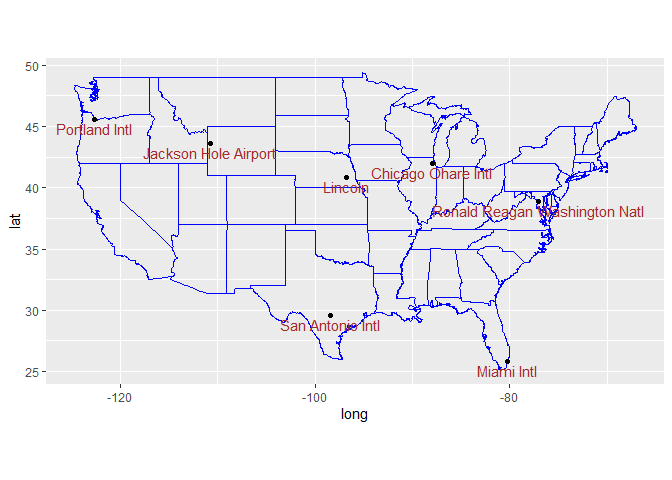
\includegraphics{tidyverse_in_class_activity_files/figure-latex/just_for_fun_with_filter-1.pdf}

\begin{Shaded}
\begin{Highlighting}[]
\CommentTok{\# Using slice function fetch the rows from 10th row to 15th row}

\CommentTok{\# Uncomment the code below to complete the response }
\NormalTok{diamonds }\SpecialCharTok{\%\textgreater{}\%} 
\FunctionTok{slice}\NormalTok{(}\DecValTok{10}\SpecialCharTok{:}\DecValTok{15}\NormalTok{)}
\end{Highlighting}
\end{Shaded}

\begin{verbatim}
## # A tibble: 6 x 10
##   carat cut       color clarity depth table price     x     y     z
##   <dbl> <ord>     <ord> <ord>   <dbl> <dbl> <int> <dbl> <dbl> <dbl>
## 1  0.23 Very Good H     VS1      59.4    61   338  4     4.05  2.39
## 2  0.3  Good      J     SI1      64      55   339  4.25  4.28  2.73
## 3  0.23 Ideal     J     VS1      62.8    56   340  3.93  3.9   2.46
## 4  0.22 Premium   F     SI1      60.4    61   342  3.88  3.84  2.33
## 5  0.31 Ideal     J     SI2      62.2    54   344  4.35  4.37  2.71
## 6  0.2  Premium   E     SI2      60.2    62   345  3.79  3.75  2.27
\end{verbatim}

\begin{Shaded}
\begin{Highlighting}[]
\CommentTok{\# Using mutate function create a normalized price value. Create a new column price\_normal}
\CommentTok{\# price\_normal is (price {-} mean(price))/ standard\_deviation(price)}
\CommentTok{\# No need to save the output dataset to a new diamonds dataset }
\CommentTok{\# Verify that the new column was created correctly by including the following line of code at the end of the pipe operation}
\CommentTok{\# filter(price == 3932 | price == 3935)}

\CommentTok{\# mutate impacts 1 column}
\NormalTok{diamonds }\SpecialCharTok{\%\textgreater{}\%}
  \FunctionTok{mutate}\NormalTok{(}\AttributeTok{normal\_price =}\NormalTok{ (price }\SpecialCharTok{{-}} \FunctionTok{mean}\NormalTok{(price))}\SpecialCharTok{/} \FunctionTok{sd}\NormalTok{(price)) }\SpecialCharTok{\%\textgreater{}\%}
\FunctionTok{filter}\NormalTok{(price }\SpecialCharTok{==} \DecValTok{3932} \SpecialCharTok{|}\NormalTok{ price }\SpecialCharTok{==} \DecValTok{3935}\NormalTok{)}
\end{Highlighting}
\end{Shaded}

\begin{verbatim}
## # A tibble: 4 x 11
##   carat cut     color clarity depth table price     x     y     z normal_price
##   <dbl> <ord>   <ord> <ord>   <dbl> <dbl> <int> <dbl> <dbl> <dbl>        <dbl>
## 1  1.01 Good    D     SI2      64      59  3932  6.28  6.34  4.04    -0.000200
## 2  0.92 Premium I     VVS1     62.4    59  3932  6.17  6.14  3.84    -0.000200
## 3  1.06 Ideal   J     SI2      61.3    57  3932  6.55  6.6   4.03    -0.000200
## 4  0.81 Ideal   E     SI1      61.9    56  3935  5.97  6.02  3.71     0.000552
\end{verbatim}

\hypertarget{the-scoped-variants-of-mutate-and-transmute-make-it-easy-to-apply-the-same-transformation-to-multiple-variables.-there-are-three-variants}{%
\paragraph{The scoped variants of mutate() and transmute() make it easy
to apply the same transformation to multiple variables. There are three
variants:}\label{the-scoped-variants-of-mutate-and-transmute-make-it-easy-to-apply-the-same-transformation-to-multiple-variables.-there-are-three-variants}}

\begin{itemize}
\item
  \_all affects every variable
\item
  \_at affects variables selected with a character vector or vars()
\item
  \_if affects variables selected with a predicate function:
\end{itemize}

\begin{Shaded}
\begin{Highlighting}[]
\CommentTok{\# using mutate\_at add $10 to the price}
\CommentTok{\# This is the syntax of mutate\_at}
\CommentTok{\# mutate\_at(.tbl, .vars, .funs, ..., .cols = NULL) }

\CommentTok{\# mutate\_at, mutate\_all \& mutate\_if are designed to impact multiple columns}

\NormalTok{increment\_10 }\OtherTok{\textless{}{-}} \ControlFlowTok{function}\NormalTok{(x) \{ x }\SpecialCharTok{+} \DecValTok{10}\NormalTok{\}}

\NormalTok{diamonds }\SpecialCharTok{\%\textgreater{}\%}
  \FunctionTok{mutate\_at}\NormalTok{(}\AttributeTok{.vars =} \FunctionTok{c}\NormalTok{(}\StringTok{"price"}\NormalTok{),}
            \AttributeTok{.funs =}\NormalTok{ increment\_10)}
\end{Highlighting}
\end{Shaded}

\begin{verbatim}
## # A tibble: 53,940 x 10
##    carat cut       color clarity depth table price     x     y     z
##    <dbl> <ord>     <ord> <ord>   <dbl> <dbl> <dbl> <dbl> <dbl> <dbl>
##  1  0.23 Ideal     E     SI2      61.5    55   336  3.95  3.98  2.43
##  2  0.21 Premium   E     SI1      59.8    61   336  3.89  3.84  2.31
##  3  0.23 Good      E     VS1      56.9    65   337  4.05  4.07  2.31
##  4  0.29 Premium   I     VS2      62.4    58   344  4.2   4.23  2.63
##  5  0.31 Good      J     SI2      63.3    58   345  4.34  4.35  2.75
##  6  0.24 Very Good J     VVS2     62.8    57   346  3.94  3.96  2.48
##  7  0.24 Very Good I     VVS1     62.3    57   346  3.95  3.98  2.47
##  8  0.26 Very Good H     SI1      61.9    55   347  4.07  4.11  2.53
##  9  0.22 Fair      E     VS2      65.1    61   347  3.87  3.78  2.49
## 10  0.23 Very Good H     VS1      59.4    61   348  4     4.05  2.39
## # ... with 53,930 more rows
\end{verbatim}

\begin{Shaded}
\begin{Highlighting}[]
\CommentTok{\# can be applied on more than one column}
\CommentTok{\# I can pass multiple functions}

\CommentTok{\# to add a new column instead of changing the price column itself}
\CommentTok{\#\textquotesingle{} to override the existing column I can put "price", rather}
\CommentTok{\#\textquotesingle{} than "new\_price"}
\NormalTok{diamonds }\SpecialCharTok{\%\textgreater{}\%}
  \FunctionTok{mutate\_at}\NormalTok{(}\AttributeTok{.vars =} \FunctionTok{c}\NormalTok{(}\StringTok{"price"}\NormalTok{),}
            \AttributeTok{.funs =} \FunctionTok{list}\NormalTok{(}\AttributeTok{new\_price =} \ControlFlowTok{function}\NormalTok{(x) x }\SpecialCharTok{+} \DecValTok{10}\NormalTok{ ))}
\end{Highlighting}
\end{Shaded}

\begin{verbatim}
## # A tibble: 53,940 x 11
##    carat cut       color clarity depth table price     x     y     z new_price
##    <dbl> <ord>     <ord> <ord>   <dbl> <dbl> <int> <dbl> <dbl> <dbl>     <dbl>
##  1  0.23 Ideal     E     SI2      61.5    55   326  3.95  3.98  2.43       336
##  2  0.21 Premium   E     SI1      59.8    61   326  3.89  3.84  2.31       336
##  3  0.23 Good      E     VS1      56.9    65   327  4.05  4.07  2.31       337
##  4  0.29 Premium   I     VS2      62.4    58   334  4.2   4.23  2.63       344
##  5  0.31 Good      J     SI2      63.3    58   335  4.34  4.35  2.75       345
##  6  0.24 Very Good J     VVS2     62.8    57   336  3.94  3.96  2.48       346
##  7  0.24 Very Good I     VVS1     62.3    57   336  3.95  3.98  2.47       346
##  8  0.26 Very Good H     SI1      61.9    55   337  4.07  4.11  2.53       347
##  9  0.22 Fair      E     VS2      65.1    61   337  3.87  3.78  2.49       347
## 10  0.23 Very Good H     VS1      59.4    61   338  4     4.05  2.39       348
## # ... with 53,930 more rows
\end{verbatim}

\begin{Shaded}
\begin{Highlighting}[]
\CommentTok{\# using mutate across, add $10 to the price. mutate across is the preferred method. }
\CommentTok{\# use mutate(across( .. rest all should be the same}
\CommentTok{\# mutate(across(.cols = everything(), .fns = NULL, ..., .names = NULL) }

\CommentTok{\#\textquotesingle{} mutate across is preferred, because it\textquotesingle{}s more specific since}
\CommentTok{\#\textquotesingle{} we are specifying the columns}
\NormalTok{diamonds }\SpecialCharTok{\%\textgreater{}\%}
  \FunctionTok{mutate}\NormalTok{(}\FunctionTok{across}\NormalTok{(}\AttributeTok{.cols =} \StringTok{"price"}\NormalTok{,}
                \AttributeTok{.fns =} \ControlFlowTok{function}\NormalTok{(x) x }\SpecialCharTok{+} \DecValTok{10}\NormalTok{))}
\end{Highlighting}
\end{Shaded}

\begin{verbatim}
## # A tibble: 53,940 x 10
##    carat cut       color clarity depth table price     x     y     z
##    <dbl> <ord>     <ord> <ord>   <dbl> <dbl> <dbl> <dbl> <dbl> <dbl>
##  1  0.23 Ideal     E     SI2      61.5    55   336  3.95  3.98  2.43
##  2  0.21 Premium   E     SI1      59.8    61   336  3.89  3.84  2.31
##  3  0.23 Good      E     VS1      56.9    65   337  4.05  4.07  2.31
##  4  0.29 Premium   I     VS2      62.4    58   344  4.2   4.23  2.63
##  5  0.31 Good      J     SI2      63.3    58   345  4.34  4.35  2.75
##  6  0.24 Very Good J     VVS2     62.8    57   346  3.94  3.96  2.48
##  7  0.24 Very Good I     VVS1     62.3    57   346  3.95  3.98  2.47
##  8  0.26 Very Good H     SI1      61.9    55   347  4.07  4.11  2.53
##  9  0.22 Fair      E     VS2      65.1    61   347  3.87  3.78  2.49
## 10  0.23 Very Good H     VS1      59.4    61   348  4     4.05  2.39
## # ... with 53,930 more rows
\end{verbatim}

\begin{Shaded}
\begin{Highlighting}[]
\CommentTok{\# using mutate\_if increase price by $10}
\CommentTok{\# mutate\_if(.tbl, .predicate, .funs, ...)}

\NormalTok{diamonds }\SpecialCharTok{\%\textgreater{}\%}
  \FunctionTok{mutate\_if}\NormalTok{(}\FunctionTok{colnames}\NormalTok{(.) }\SpecialCharTok{==} \StringTok{"price"}\NormalTok{,}
            \AttributeTok{.funs =} \ControlFlowTok{function}\NormalTok{(x) x }\SpecialCharTok{+} \DecValTok{10}\NormalTok{)}
\end{Highlighting}
\end{Shaded}

\begin{verbatim}
## # A tibble: 53,940 x 10
##    carat cut       color clarity depth table price     x     y     z
##    <dbl> <ord>     <ord> <ord>   <dbl> <dbl> <dbl> <dbl> <dbl> <dbl>
##  1  0.23 Ideal     E     SI2      61.5    55   336  3.95  3.98  2.43
##  2  0.21 Premium   E     SI1      59.8    61   336  3.89  3.84  2.31
##  3  0.23 Good      E     VS1      56.9    65   337  4.05  4.07  2.31
##  4  0.29 Premium   I     VS2      62.4    58   344  4.2   4.23  2.63
##  5  0.31 Good      J     SI2      63.3    58   345  4.34  4.35  2.75
##  6  0.24 Very Good J     VVS2     62.8    57   346  3.94  3.96  2.48
##  7  0.24 Very Good I     VVS1     62.3    57   346  3.95  3.98  2.47
##  8  0.26 Very Good H     SI1      61.9    55   347  4.07  4.11  2.53
##  9  0.22 Fair      E     VS2      65.1    61   347  3.87  3.78  2.49
## 10  0.23 Very Good H     VS1      59.4    61   348  4     4.05  2.39
## # ... with 53,930 more rows
\end{verbatim}

\begin{Shaded}
\begin{Highlighting}[]
\CommentTok{\# using mutate function add a new column to the diamonds dataset called discounted\_price to capture discounted price depending on the cut of the diamond.  }
\CommentTok{\# if "Fair" {-} price*.90, if "Good" {-} price*.85, if "Very Good" {-} price*.80, if "Premium" {-} price*.75, if "Ideal" {-} price*.75}

\CommentTok{\# using case statements within mutate}
\NormalTok{diamonds }\SpecialCharTok{\%\textgreater{}\%}
  \FunctionTok{mutate}\NormalTok{(}\AttributeTok{discounted\_price =} \FunctionTok{case\_when}\NormalTok{(cut }\SpecialCharTok{==} \StringTok{"Fair"} \SpecialCharTok{\textasciitilde{}} \FloatTok{0.9}\SpecialCharTok{*}\NormalTok{price,}
\NormalTok{                                      cut }\SpecialCharTok{==} \StringTok{"Good"} \SpecialCharTok{\textasciitilde{}} \FloatTok{0.85}\SpecialCharTok{*}\NormalTok{price,}
\NormalTok{                                      cut }\SpecialCharTok{==} \StringTok{"Very Good"} \SpecialCharTok{\textasciitilde{}} \FloatTok{0.8}\SpecialCharTok{*}\NormalTok{price,}
\NormalTok{                                      cut }\SpecialCharTok{==} \StringTok{"Premium"} \SpecialCharTok{\textasciitilde{}} \FloatTok{0.75}\SpecialCharTok{*}\NormalTok{price,}
                                      \ConstantTok{TRUE} \SpecialCharTok{\textasciitilde{}} \FloatTok{0.75}\SpecialCharTok{*}\NormalTok{price))}
\end{Highlighting}
\end{Shaded}

\begin{verbatim}
## # A tibble: 53,940 x 11
##    carat cut       color clarity depth table price     x     y     z discounte~1
##    <dbl> <ord>     <ord> <ord>   <dbl> <dbl> <int> <dbl> <dbl> <dbl>       <dbl>
##  1  0.23 Ideal     E     SI2      61.5    55   326  3.95  3.98  2.43        244.
##  2  0.21 Premium   E     SI1      59.8    61   326  3.89  3.84  2.31        244.
##  3  0.23 Good      E     VS1      56.9    65   327  4.05  4.07  2.31        278.
##  4  0.29 Premium   I     VS2      62.4    58   334  4.2   4.23  2.63        250.
##  5  0.31 Good      J     SI2      63.3    58   335  4.34  4.35  2.75        285.
##  6  0.24 Very Good J     VVS2     62.8    57   336  3.94  3.96  2.48        269.
##  7  0.24 Very Good I     VVS1     62.3    57   336  3.95  3.98  2.47        269.
##  8  0.26 Very Good H     SI1      61.9    55   337  4.07  4.11  2.53        270.
##  9  0.22 Fair      E     VS2      65.1    61   337  3.87  3.78  2.49        303.
## 10  0.23 Very Good H     VS1      59.4    61   338  4     4.05  2.39        270.
## # ... with 53,930 more rows, and abbreviated variable name 1: discounted_price
\end{verbatim}

\begin{Shaded}
\begin{Highlighting}[]
\CommentTok{\# sort the diamonds dataset by cut column and select, price, cut and depth columns }

\CommentTok{\# arrange is used to sort}
\FunctionTok{view}\NormalTok{(diamonds }\SpecialCharTok{\%\textgreater{}\%}
  \FunctionTok{arrange}\NormalTok{(}\FunctionTok{desc}\NormalTok{(cut)) }\SpecialCharTok{\%\textgreater{}\%} \CommentTok{\# desc is used to arrange in descending order}
  \FunctionTok{select}\NormalTok{(price, cut, depth))}
\end{Highlighting}
\end{Shaded}

\begin{Shaded}
\begin{Highlighting}[]
\CommentTok{\# Using the diamonds dataset and summarize function, calculate the mean\_price, mean\_depth, and variance\_x (using x variable)(group by cut)}
\NormalTok{diamonds }\SpecialCharTok{\%\textgreater{}\%}
  \FunctionTok{group\_by}\NormalTok{(cut) }\SpecialCharTok{\%\textgreater{}\%}
  \FunctionTok{summarise}\NormalTok{(}\AttributeTok{mean\_price =} \FunctionTok{mean}\NormalTok{(price),}
            \AttributeTok{mean\_depth =} \FunctionTok{mean}\NormalTok{(depth),}
            \AttributeTok{variance\_x =} \FunctionTok{sd}\NormalTok{(x)}\SpecialCharTok{\^{}}\DecValTok{2}\NormalTok{)}
\end{Highlighting}
\end{Shaded}

\begin{verbatim}
## # A tibble: 5 x 4
##   cut       mean_price mean_depth variance_x
##   <ord>          <dbl>      <dbl>      <dbl>
## 1 Fair           4359.       64.0      0.930
## 2 Good           3929.       62.4      1.12 
## 3 Very Good      3982.       61.8      1.21 
## 4 Premium        4584.       61.3      1.41 
## 5 Ideal          3458.       61.7      1.13
\end{verbatim}

\begin{Shaded}
\begin{Highlighting}[]
\CommentTok{\# Complete the code below to generate a dataset containing the datetime and price of a fictitious cryptocoin with a consistent hourly increase of 0.001 in value.)}
\FunctionTok{library}\NormalTok{(lubridate)}
\end{Highlighting}
\end{Shaded}

\begin{verbatim}
## Warning: package 'lubridate' was built under R version 4.1.3
\end{verbatim}

\begin{verbatim}
## 
## Attaching package: 'lubridate'
\end{verbatim}

\begin{verbatim}
## The following objects are masked from 'package:base':
## 
##     date, intersect, setdiff, union
\end{verbatim}

\begin{Shaded}
\begin{Highlighting}[]
\NormalTok{total\_hours }\OtherTok{\textless{}{-}} \FunctionTok{ymd\_hms}\NormalTok{(}\StringTok{"2023{-}03{-}01 00:00:00"}\NormalTok{) }\SpecialCharTok{+} \DecValTok{0}\SpecialCharTok{:}\DecValTok{200}\SpecialCharTok{*}\DecValTok{24} \CommentTok{\# Some 200 random days}
\CommentTok{\# Uncomment the line of code below to complete a mutate \& a cumsum function and create a variable that stores the cumulative price increase. Utilize a rnorm with a mean of 0.001 and a standard deviation of 0.01}

\NormalTok{crypto\_price }\OtherTok{\textless{}{-}} \FunctionTok{as.tibble}\NormalTok{(total\_hours) }\SpecialCharTok{\%\textgreater{}\%} 
  \FunctionTok{mutate}\NormalTok{(}\AttributeTok{price =} \FloatTok{0.07} \SpecialCharTok{+} \FunctionTok{cumsum}\NormalTok{(}\FunctionTok{rnorm}\NormalTok{(}\FunctionTok{n}\NormalTok{(), }\AttributeTok{mean =} \FloatTok{0.001}\NormalTok{, }\AttributeTok{sd =} \FloatTok{0.01}\NormalTok{)))}
\end{Highlighting}
\end{Shaded}

\begin{verbatim}
## Warning: `as.tibble()` was deprecated in tibble 2.0.0.
## i Please use `as_tibble()` instead.
## i The signature and semantics have changed, see `?as_tibble`.
\end{verbatim}

\begin{Shaded}
\begin{Highlighting}[]
\FunctionTok{plot}\NormalTok{(}\AttributeTok{x =}\NormalTok{ crypto\_price}\SpecialCharTok{$}\NormalTok{value, }\AttributeTok{y =}\NormalTok{ crypto\_price}\SpecialCharTok{$}\NormalTok{price)}
\end{Highlighting}
\end{Shaded}

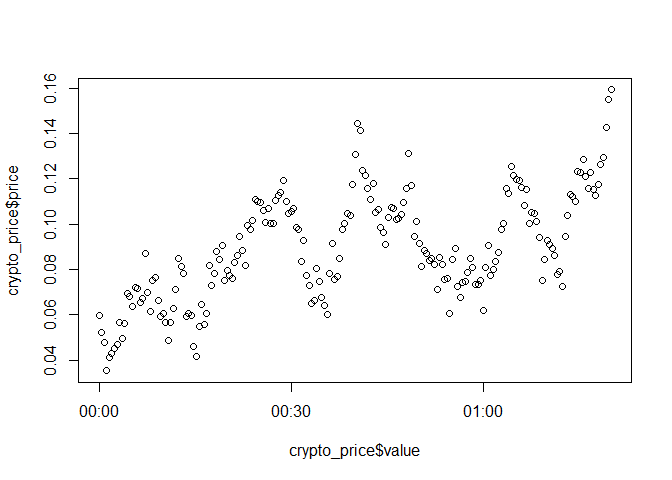
\includegraphics{tidyverse_in_class_activity_files/figure-latex/Q22. Create a cumulative hourly increase of 0.001 in the average crypto price.-1.pdf}

\begin{Shaded}
\begin{Highlighting}[]
\CommentTok{\# create a union of the diamonds1 and diamonds2 datasets}
\CommentTok{\# Look at the cheatsheet for understanding these functions. Also, please pay attention to the intersect function you are using. }
\NormalTok{diamonds1 }\OtherTok{\textless{}{-}}\NormalTok{ diamonds[diamonds}\SpecialCharTok{$}\NormalTok{depth }\SpecialCharTok{\textless{}} \DecValTok{50}\NormalTok{,]}
\NormalTok{diamonds2 }\OtherTok{\textless{}{-}}\NormalTok{ diamonds[diamonds}\SpecialCharTok{$}\NormalTok{depth }\SpecialCharTok{\textless{}} \DecValTok{55}\NormalTok{,]}

\NormalTok{diamonds1 }\SpecialCharTok{\%\textgreater{}\%}
\NormalTok{  dplyr}\SpecialCharTok{::}\FunctionTok{union}\NormalTok{(diamonds2)}
\end{Highlighting}
\end{Shaded}

\begin{verbatim}
## # A tibble: 22 x 10
##    carat cut   color clarity depth table price     x     y     z
##    <dbl> <ord> <ord> <ord>   <dbl> <dbl> <int> <dbl> <dbl> <dbl>
##  1  1    Fair  G     SI1      43      59  3634  6.32  6.27  3.97
##  2  1    Fair  G     VS2      44      53  4032  6.31  6.24  4.12
##  3  1.09 Ideal J     VS2      43      54  4778  6.53  6.55  4.12
##  4  0.96 Fair  E     SI2      53.1    63  2815  6.73  6.65  3.55
##  5  0.98 Fair  E     SI2      53.3    67  2855  6.82  6.74  3.61
##  6  1.02 Fair  I     SI1      53      63  2856  6.84  6.77  3.66
##  7  1.08 Fair  E     SI1      53.8    63  4790  6.99  6.81  3.71
##  8  1.26 Fair  G     SI2      53.2    61  4966  7.44  7.36  3.94
##  9  1.43 Fair  I     VS1      50.8    60  6727  7.73  7.25  3.93
## 10  0.31 Fair  E     VS2      54.2    63   814  4.61  4.51  2.47
## # ... with 12 more rows
\end{verbatim}

\begin{Shaded}
\begin{Highlighting}[]
\CommentTok{\# eliminates duplication}

\CommentTok{\# if we want to combine datasets even with duplicates we use union all}
\end{Highlighting}
\end{Shaded}

\begin{Shaded}
\begin{Highlighting}[]
\CommentTok{\# create a intersection of the diamonds1 and diamonds2 datasets}
\NormalTok{diamonds1 }\SpecialCharTok{\%\textgreater{}\%}
\NormalTok{  dplyr}\SpecialCharTok{::}\FunctionTok{intersect}\NormalTok{(diamonds2)}
\end{Highlighting}
\end{Shaded}

\begin{verbatim}
## # A tibble: 3 x 10
##   carat cut   color clarity depth table price     x     y     z
##   <dbl> <ord> <ord> <ord>   <dbl> <dbl> <int> <dbl> <dbl> <dbl>
## 1  1    Fair  G     SI1        43    59  3634  6.32  6.27  3.97
## 2  1    Fair  G     VS2        44    53  4032  6.31  6.24  4.12
## 3  1.09 Ideal J     VS2        43    54  4778  6.53  6.55  4.12
\end{verbatim}

\begin{Shaded}
\begin{Highlighting}[]
\CommentTok{\# displays common rows}
\end{Highlighting}
\end{Shaded}

\begin{Shaded}
\begin{Highlighting}[]
\CommentTok{\# use setdiff function of dplyr to find the rows that differ diamonds1 and diamonds2 datasets}
\NormalTok{diamonds2 }\SpecialCharTok{\%\textgreater{}\%}
\NormalTok{  dplyr}\SpecialCharTok{::}\FunctionTok{setdiff}\NormalTok{(diamonds1)}
\end{Highlighting}
\end{Shaded}

\begin{verbatim}
## # A tibble: 19 x 10
##    carat cut   color clarity depth table price     x     y     z
##    <dbl> <ord> <ord> <ord>   <dbl> <dbl> <int> <dbl> <dbl> <dbl>
##  1  0.96 Fair  E     SI2      53.1    63  2815  6.73  6.65  3.55
##  2  0.98 Fair  E     SI2      53.3    67  2855  6.82  6.74  3.61
##  3  1.02 Fair  I     SI1      53      63  2856  6.84  6.77  3.66
##  4  1.08 Fair  E     SI1      53.8    63  4790  6.99  6.81  3.71
##  5  1.26 Fair  G     SI2      53.2    61  4966  7.44  7.36  3.94
##  6  1.43 Fair  I     VS1      50.8    60  6727  7.73  7.25  3.93
##  7  0.31 Fair  E     VS2      54.2    63   814  4.61  4.51  2.47
##  8  0.3  Fair  E     VVS2     51      67   945  4.67  4.62  2.37
##  9  0.31 Fair  D     VVS2     54.2    65   997  4.61  4.58  2.49
## 10  0.35 Fair  F     VVS1     54.6    59  1011  4.85  4.79  2.63
## 11  0.35 Fair  D     VVS2     53.2    62  1011  4.87  4.8   2.57
## 12  0.34 Fair  E     VVS1     54      56  1012  4.8   4.76  2.58
## 13  0.25 Fair  F     SI2      54.4    64  1013  4.3   4.23  2.32
## 14  0.37 Fair  F     IF       52.3    61  1166  4.96  4.91  2.58
## 15  0.56 Fair  H     VS2      52.7    70  1293  5.71  5.57  2.97
## 16  0.53 Good  D     SI2      54.3    65  1352  5.46  5.51  2.98
## 17  0.7  Fair  D     SI1      52.2    65  1895  6.04  5.99  3.14
## 18  0.73 Fair  F     SI2      53.4    65  2164  6.19  6.15  3.3 
## 19  0.78 Fair  H     VS2      54.7    67  2691  6.25  6.15  3.4
\end{verbatim}

\begin{Shaded}
\begin{Highlighting}[]
\CommentTok{\# shows records that are not present in diamonds2}
\end{Highlighting}
\end{Shaded}


\end{document}
